\chapterold{L'operatore GOTO}

L'operatore GOTO e' generalmente considerato un "anti-pattern", cfr. [Edgar Dijkstra, \IT{Go To Statement Considered Harmful} (1968)\footnote{\url{http://yurichev.com/mirrors/Dijkstra68.pdf}}].
Ciononostante puo' essere usato ragionevolmente, [Donald E. Knuth, \IT{Structured Programming with go to Statements} (1974)\footnote{\url{http://yurichev.com/mirrors/KnuthStructuredProgrammingGoTo.pdf}}]
\footnote{[\CNotes] ha anche alcuni esempi}.

Ecco un esempio molto semplice:

\lstinputlisting{patterns/065_GOTO/goto.c}

...e quello che otteniamo con MSVC 2012:

\lstinputlisting[caption=MSVC 2012]{patterns/065_GOTO/MSVC_goto.asm}

Lo statement \IT{goto} e' stato semplicemente sostituito con un'istruzione \JMP, che ha lo stesso effetto: un salto non condizionale
ad un altro punto del codice.
La seconda \printf puo' essere eseguita soltanto con l'intervento umano, utilizzando un debugger o patchando manualmente il codice.

\par

\clearpage

Questo esempio puo' infatti essere utile come semplice esercizio di patching. Apriamo l'eseguibile con Hiew:

\begin{figure}[H]
\centering
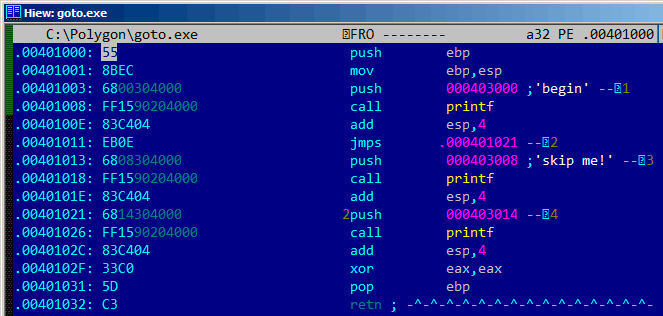
\includegraphics[scale=\FigScale]{patterns/065_GOTO/hiew1.png}
\caption{Hiew}
\label{fig:goto_hiew1}
\end{figure}

\clearpage
Posizioniamo il cursore all'indirizzo di \JMP (\TT{0x410}), 
premiamo F3 (edit), premiamo due volte zero, cosi da modificare l'opcode in \TT{EB 00}:

\begin{figure}[H]
\centering
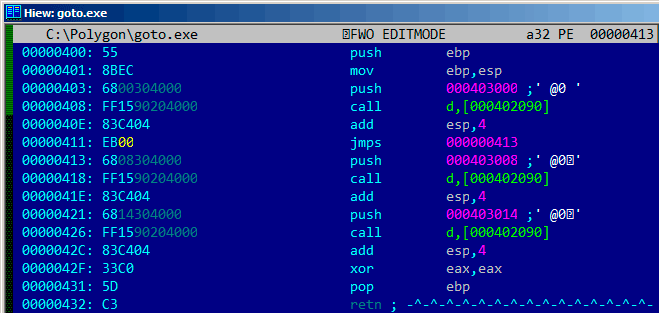
\includegraphics[scale=\FigScale]{patterns/065_GOTO/hiew2.png}
\caption{Hiew}
\label{fig:goto_hiew2}
\end{figure}

Il secondo byte dell'opcode di \JMP denota l'offset relativo per il salto, 0 significa il punto subito dopo l'istruzione corrente.

Adesso \JMP non saltera' la seconda chiamata a \printf.

Premiamo F9 (save) e usciamo da Hiew. Dopo aver eseguito il programma dovremmo vedere questo:

\begin{figure}[H]
\centering
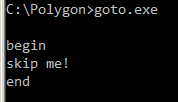
\includegraphics[scale=\NormalScale]{patterns/065_GOTO/result.png}
\caption{Patched executable output}
\label{fig:goto_result}
\end{figure}

Lo stesso risultato puo' essere ottenuto sostituendo l'istruzione \JMP con 2 istruzioni \NOP.

\NOP ha opcode \TT{0x90} ed e' lunga 1 byte, quindi servono 2 istruzioni per rimpiazzare \JMP (che e' lunga 2 byte).

\sectionold{Dead code}

In termini di compilatore, la seconda chiamata a \printf e' anche detta \q{dead code} (codice morto).
Sta a significare che quel codice non sara' mai eseguito. Se proviamo a compilare l'esempio con le ottimizzazioni, il compilatore
rimuove completamente il \q{dead code}, di cui non resta traccia:

\lstinputlisting[caption=\Optimizing MSVC 2012]{patterns/065_GOTO/MSVC_goto_Ox.asm}

Il compilatore si e' pero' dimenticato di rimuovere la stringa \q{skip me!}.

%Note: cl "/Ox" option for maximum optimisation does get rid of "skip me" string as well

\sectionold{\Exercise}

% TODO debugger example can fit here

Provate ad ottenere lo stesso risultato utilizzato il vostro compilatore e debugger preferito.
